
\section{Основная часть}

    \subsection{Определение модели}

        Модель Hassell имеет следующую математическая запись:

        \[x_{t+1} = \frac{\alpha x_t^2}{(\beta + x_t)^6}\]

        где \(x_i\) --- количество особей в поколении с номером i. Параметр \(\alpha\) определяет скорость роста популяции, а параметр \(\beta\) определяет несущую способность окружающей среды.
    
    \subsection{Частный случай}
    
        Зафиксируем параметр \(\alpha = 1\). Параметр \(\beta\) изменяется в диапазоне \([0; 0.6]\). Также запишем уравнение в таком виде:

        \[x = \frac{\alpha x^2}{(\beta + x)^6}\]
    
        \[1 = \frac{\alpha x}{(\beta + x)^6}\]

        \[\alpha x = (\beta + x)^6\]

        Теперь можно построить графики функций \(y = \alpha x\) и \(y = (\beta + x)^6\). В зависимости от значений параметра \(\beta\) уравнение может иметь ноль, одну или две общие точки. На рисунках (\ref{mainIntersect}), (\ref{mainTouch}), (\ref{mainOver}) можно увидеть все возможные варианты.
        
        \begin{figure}
            \centering
            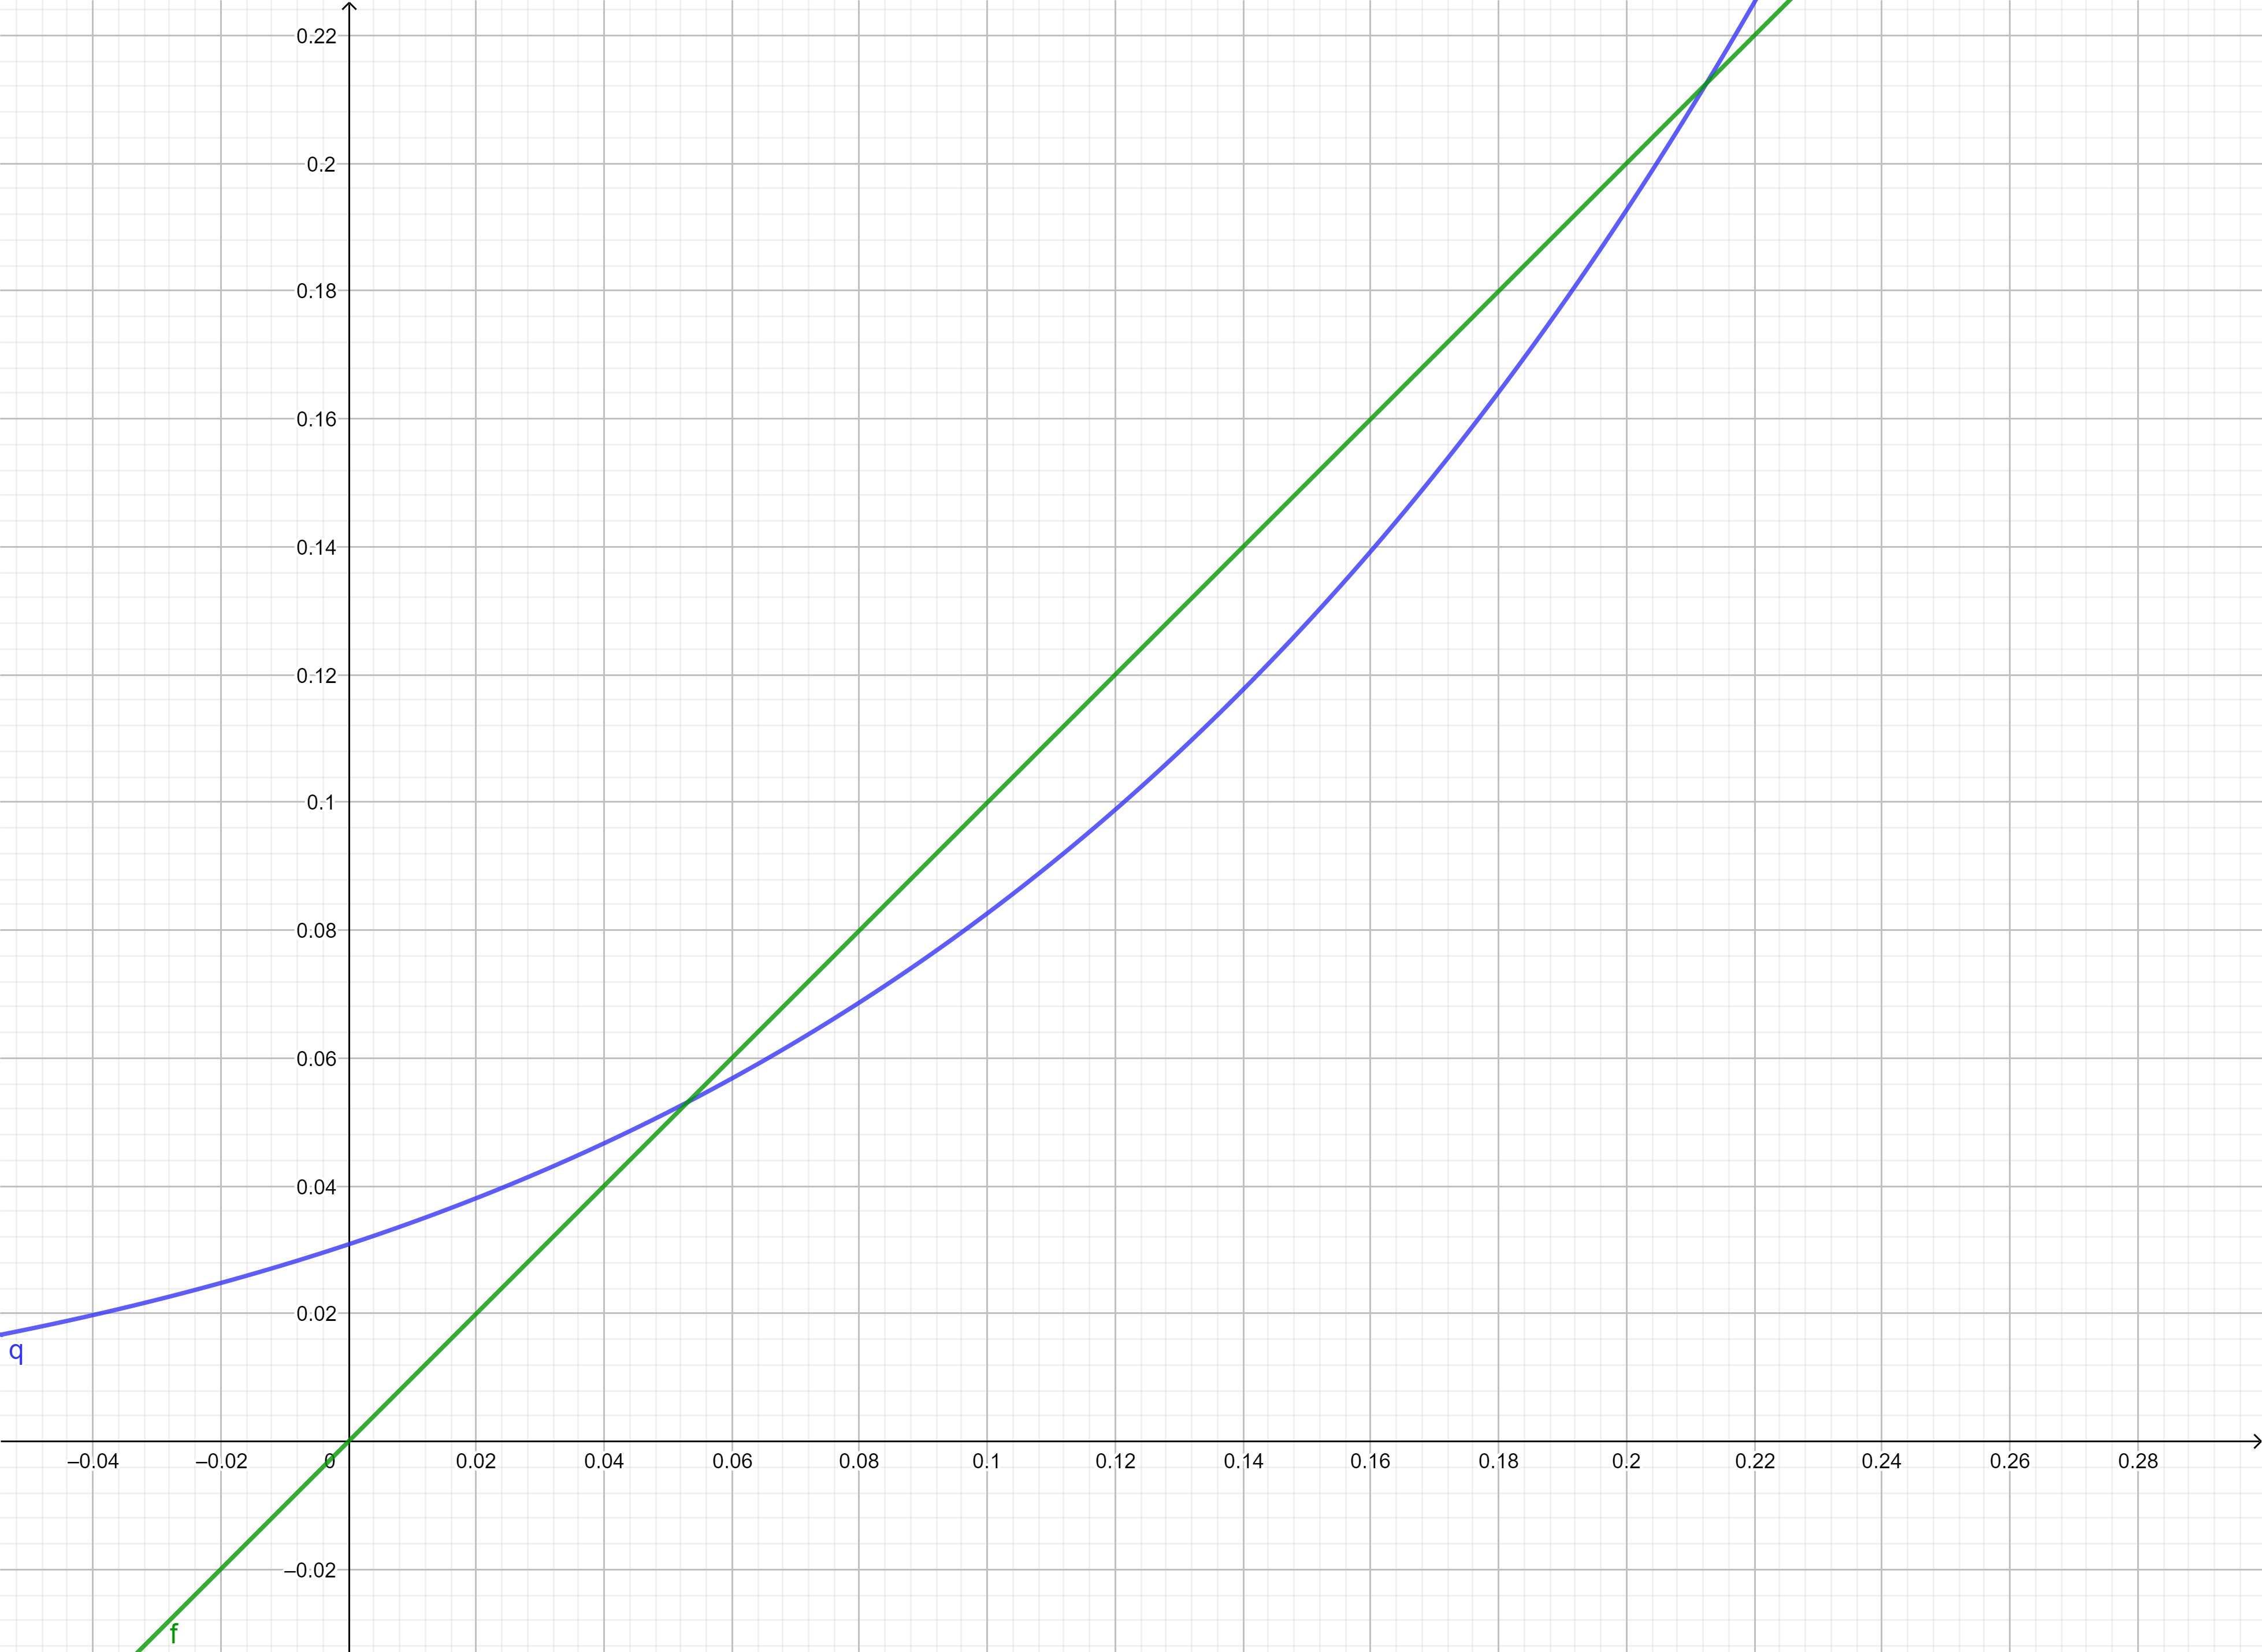
\includegraphics[width=\textwidth]{images/main_intersect.jpg}

            \captionsetup{justification=centering}
            \caption{\(\beta < 0.582355932\)}
            \label{mainIntersect}
        \end{figure}

        \begin{figure}
            \centering
            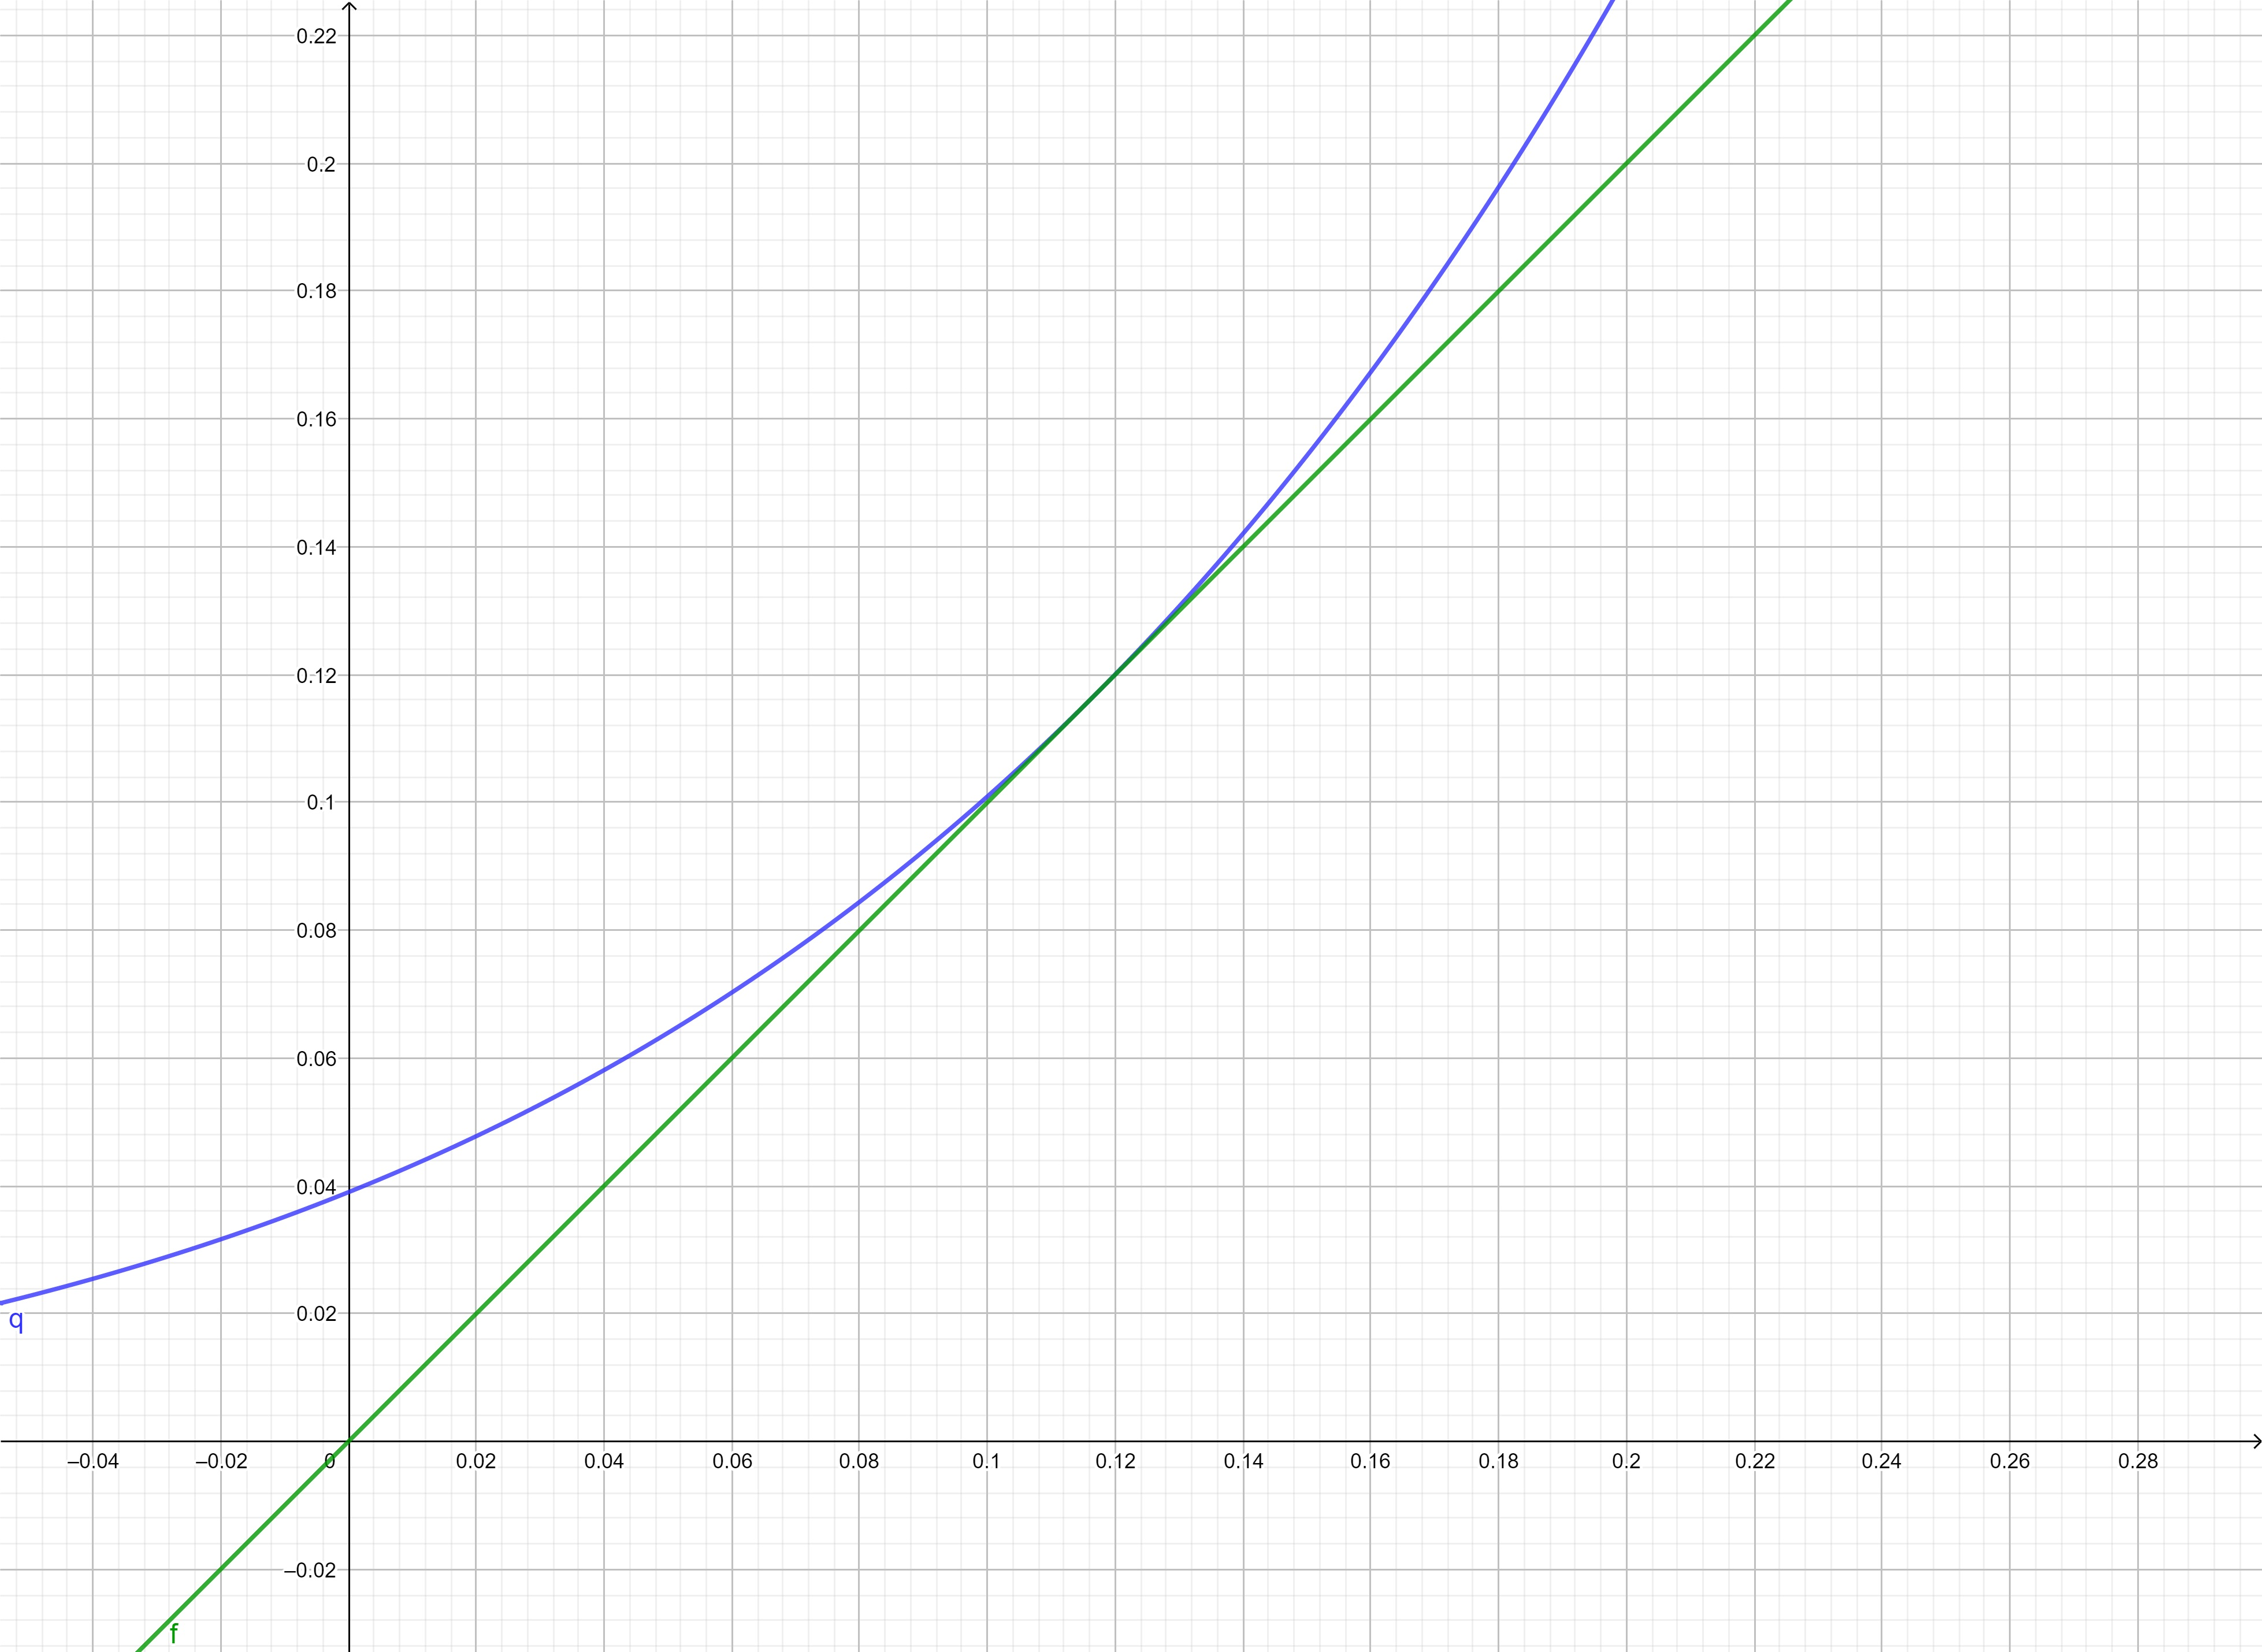
\includegraphics[width=\textwidth]{images/main_touch.jpg}

            \captionsetup{justification=centering}
            \caption{\(\beta \approx 0.582355932\)}
            \label{mainTouch}
        \end{figure}

        \begin{figure}
            \centering
            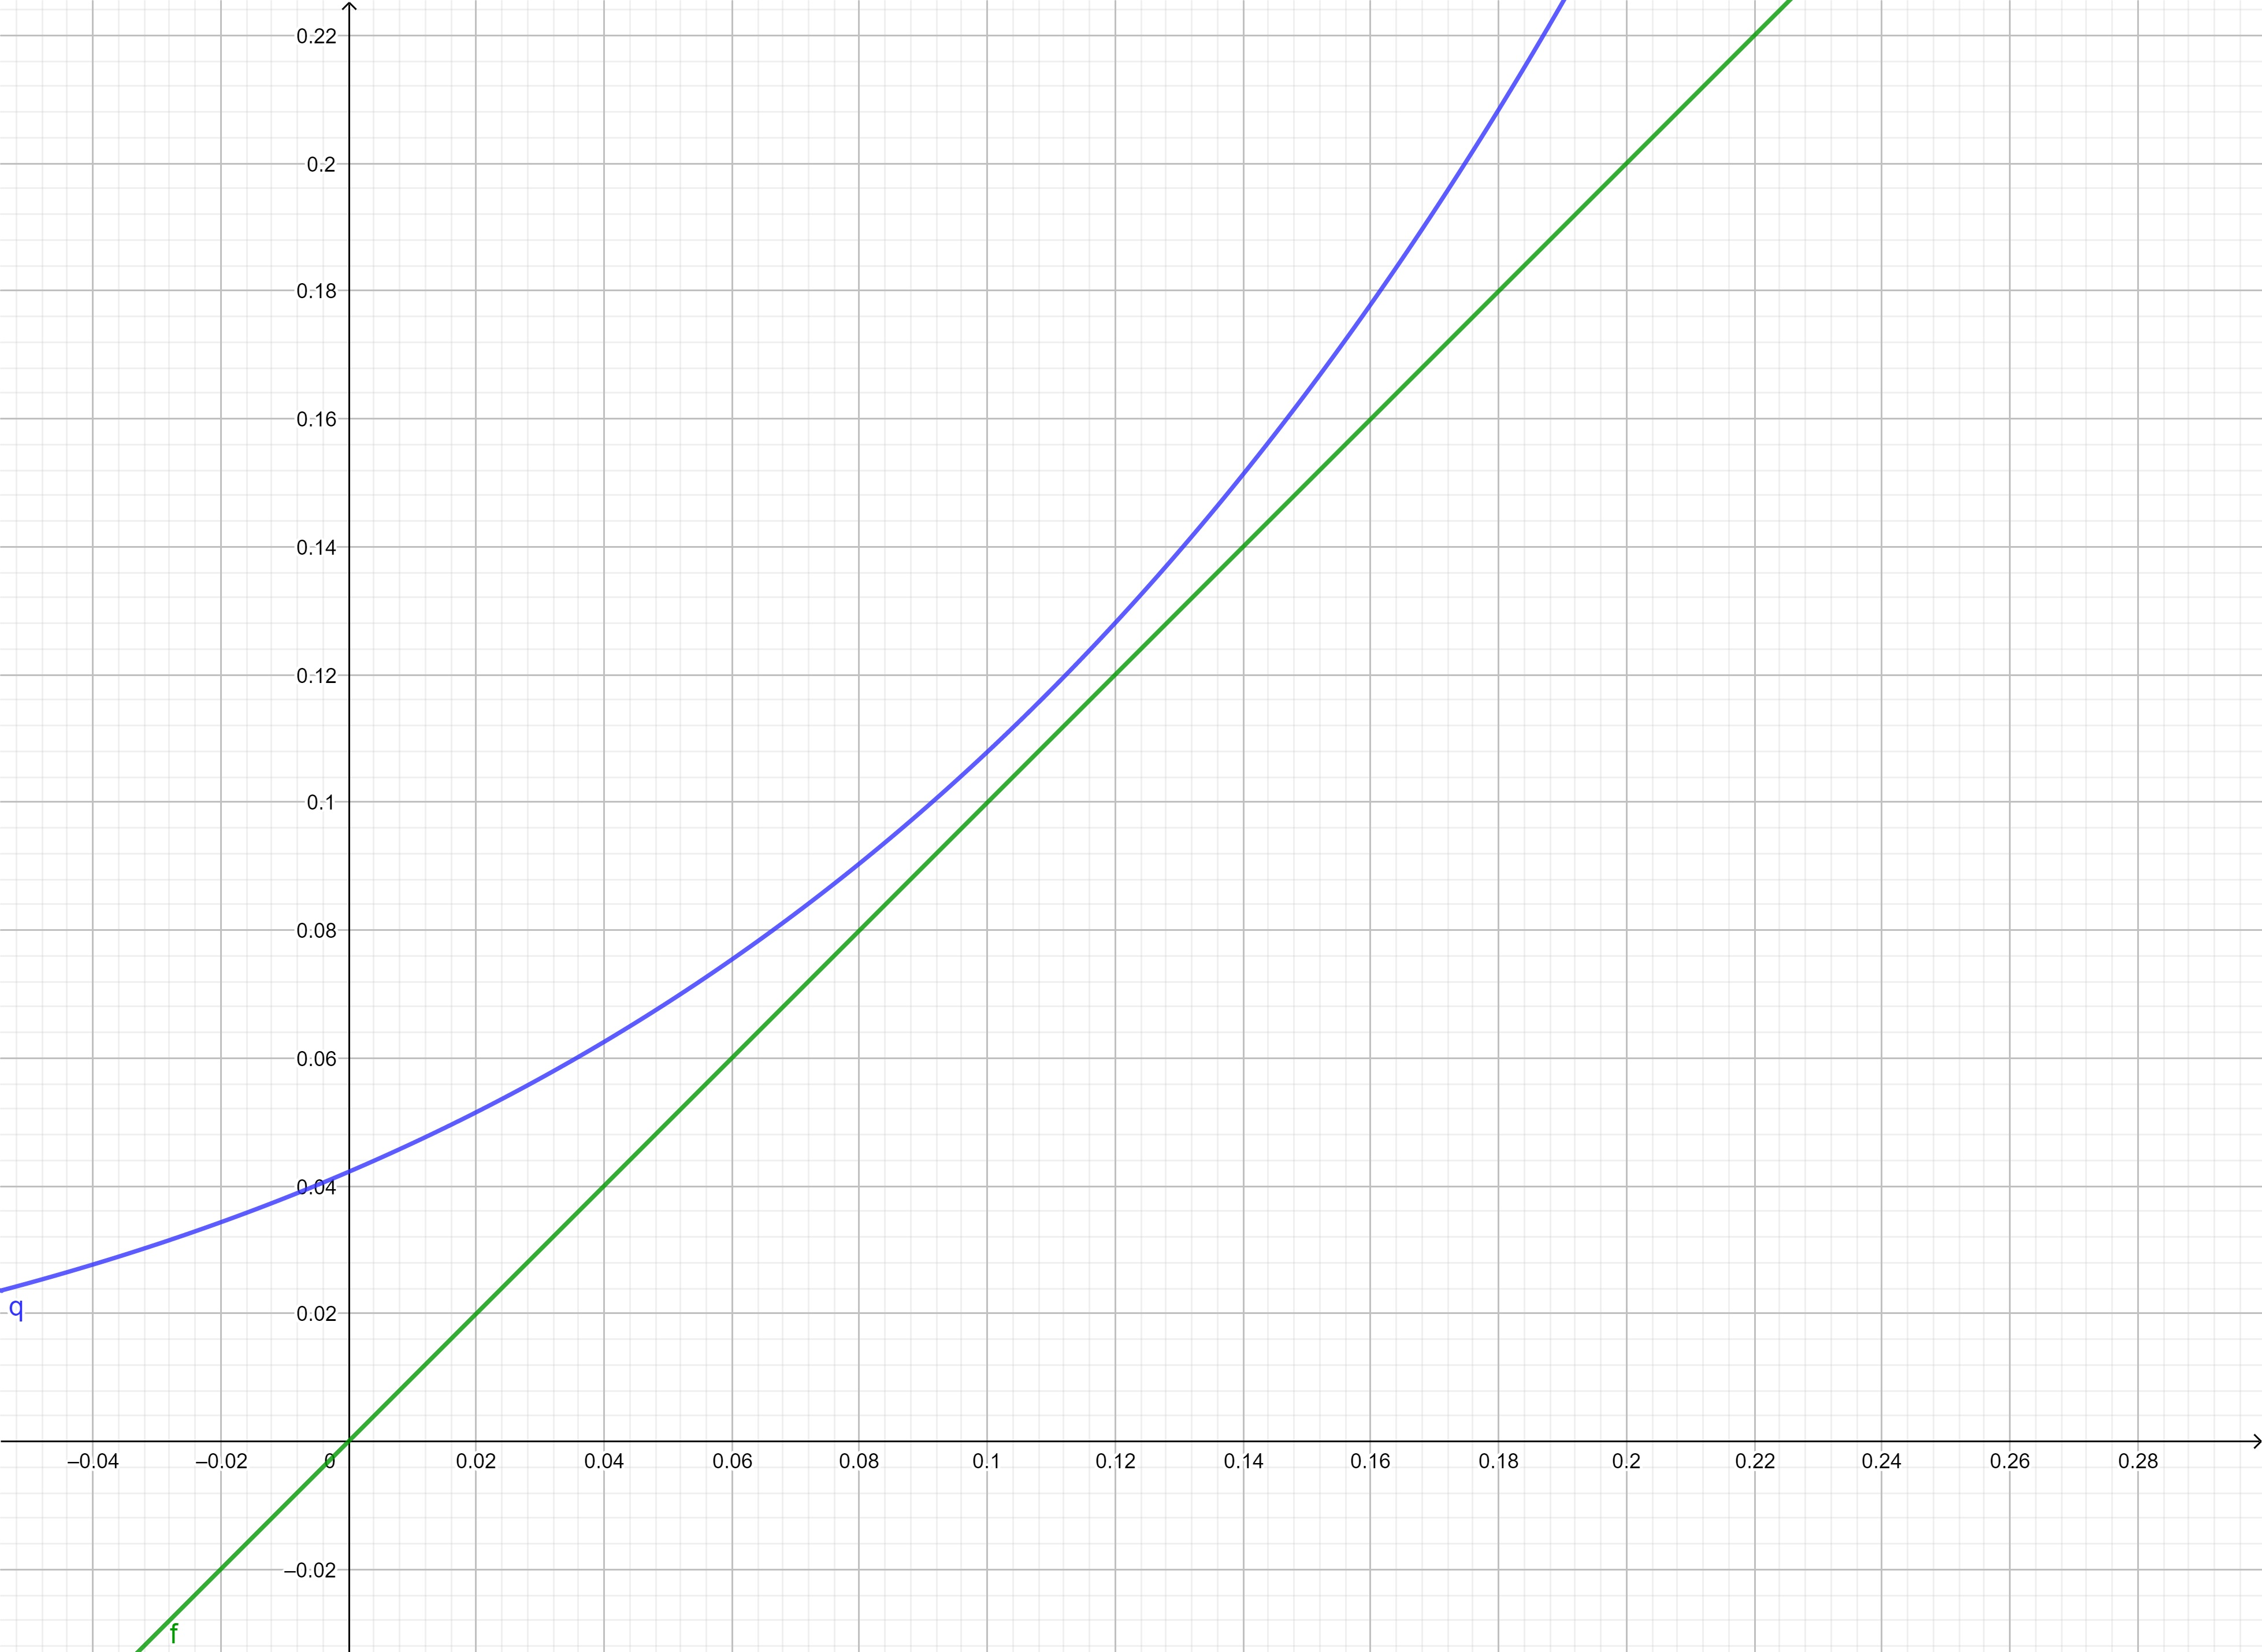
\includegraphics[width=\textwidth]{images/main_over.jpg}

            \captionsetup{justification=centering}
            \caption{\(\beta > 0.582355932\)}
            \label{mainOver}
        \end{figure}

        Аналитически это уравнение не решается. Для нахождения корней я буду использовать метод Ньютона. В зависимости от конкретных значений параметра \(\beta\) данное уравнение может иметь от одного до трех корней.

    \subsection{Временные ряды}

        Для анализа системы можно использовать временные ряды. Временной ряд позволяет наглядно показать как с течением времени изменяется численность популяции.

        Далее рассмотрим подробнее все возможные ситуации. Для этого давайте зафиксируем параметры следующим образом: \(\alpha = 1, \beta = 0.56\). 

        На графике (\ref{time_series_x_0_04_b_0_56}) мы видим, что временной ряд сходятся к нулю. В биологическом смысле это означает, что популяция с теченеим времени вымирает.
    
        \begin{figure}[h!]
            \centering
            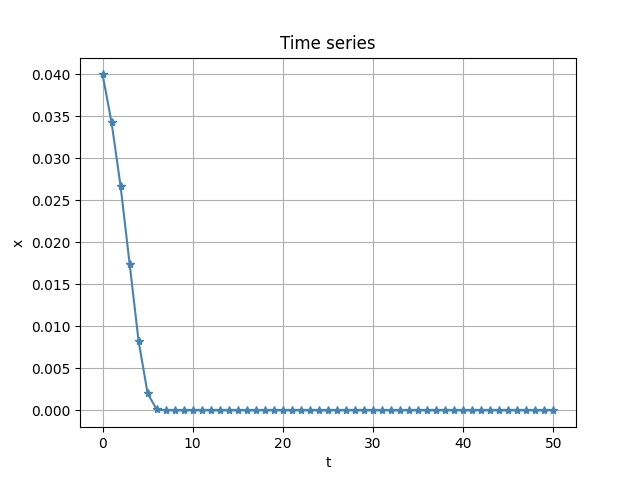
\includegraphics[width=\textwidth]{time_series_x_0_04_b_0_56.jpeg}

            \captionsetup{justification=centering}
            \caption{\(x_0 = 0.04; \beta = 0.56\)}
            \label{time_series_x_0_04_b_0_56}
        \end{figure}

        На графике (\ref{time_series_x_0_06_b_0_56}) видно, что при начальных условиях \(x = 0.06, \beta = 0.56\) популяция очень быстро растет до некоторого предела. После достижения данного предела рост численности популяции прекращается. Это значит, что популяция с течением времени стабилизируется.
    
        \begin{figure}[h!]
            \centering
            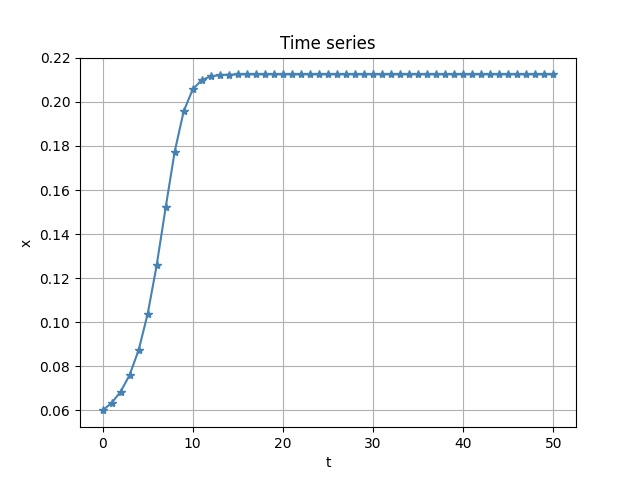
\includegraphics[width=\textwidth]{time_series_x_0_06_b_0_56.jpeg}

            \captionsetup{justification=centering}
            \caption{\(x_0 = 0.06; \beta = 0.56\)}
            \label{time_series_x_0_06_b_0_56}
        \end{figure}

        Очень похожую ситуацию мы можем наблюдать на графике (\ref{time_series_x_0_3_b_0_56}). Значения тоже сходятся к устойчивому равновесию. Т.е. численность популяции снова стабилизируется.
    
        \begin{figure}[h!]
            \centering
            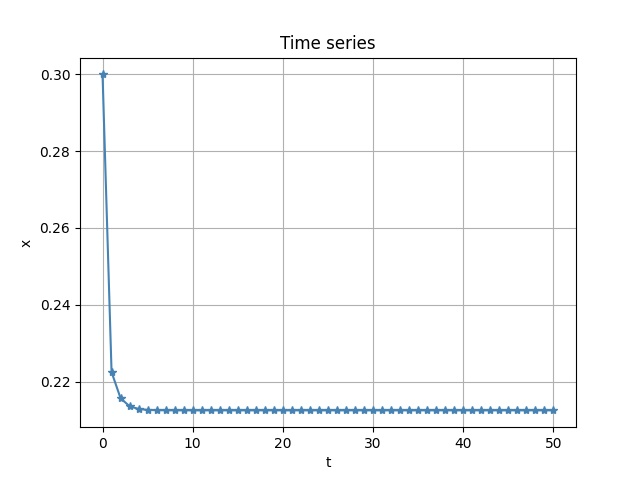
\includegraphics[width=\textwidth]{time_series_x_0_3_b_0_56.jpeg}

            \captionsetup{justification=centering}
            \caption{\(x_0 = 0.3; \beta = 0.55\)}
            \label{time_series_x_0_3_b_0_56}
        \end{figure}

        Но если начальный размер популяции слишком большой, то может произойти вымирание. Такая ситуация изображена на графике (\ref{time_series_x_1_2_b_0_56}).
    
        \begin{figure}[h!]
            \centering
            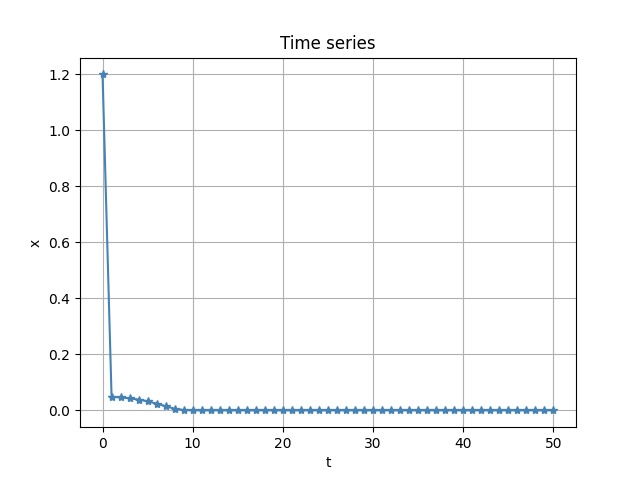
\includegraphics[width=\textwidth]{time_series_x_1_2_b_0_56.jpeg}

            \captionsetup{justification=centering}
            \caption{\(x_0 = 1.2; \beta = 0.56\)}
            \label{time_series_x_1_2_b_0_56}
        \end{figure}

    \subsection{График бифуркации}

    \subsection{Лестница Ламери}

    \subsection{Показатели Ляпунова}

    \subsection{Недоделанная карта}